\documentclass[a4paper]{article}

\makeatletter
\renewcommand\paragraph{\@startsection{paragraph}{4}{\z@}%
  {-3.25ex\@plus -1ex \@minus -.2ex}%
  {1.5ex \@plus .2ex}%
  {\normalfont\normalsize\bfseries}}
\renewcommand\subparagraph{\@startsection{subparagraph}{5}{\z@}%
  {-3.25ex\@plus -1ex \@minus -.2ex}%
  {1.5ex \@plus .2ex}%
  {\normalfont\normalsize\bfseries}}
\makeatother

\usepackage{fullpage}
\usepackage{graphicx}
\usepackage{wrapfig}
\usepackage{enumitem}
\usepackage[font=small,labelfont=bf]{caption}
\graphicspath{{./images/}}
\pagenumbering{arabic}
\begin{document}

\begin{titlepage}

\begin{center}

Delft University of Technology\\
Faculty of Electrical Engineering, Mathematics and Computer Science\\[3cm]
\huge \bf{Developing a Child-Driven \\ Online Learning Environment \\ for Third-World Countries}\\[15cm]
\end{center}

\large \noindent 
Joris Albeda, Chiel Huurdeman, Elmer Jacobs and Zmitser Zhaleznichenka\\
\{J.J.W.Albeda, C.Huurdeman, E.J.Jacobs, D.V.Zhaleznichenka\}@student.tudelft.nl\\

\noindent\today

\end{titlepage}

\setcounter{secnumdepth}{3}

\abstract \emph{This is the final report for the IN4179 Intelligent User Experience Engineering course. This project involved the design of an online learning environment for children in third-world countries, based on the ideas of Sugata Mitra. The environment employs an avatar of a teacher communicating with the children to facilitate the educational process. Using a teacher avatar, we try to exploit the so-called �grannie effect� to let young
children learn by themselves in groups using computers connected to the Internet.}

\section{Introduction}

There are many problems related to the education process in third-world countries. One of the most important ones is the lack of experienced teachers and good study materials. This problem attracts the attention of many specialists in education who suggest solutions aimed at decreasing the role of a teacher and forcing the children to learn themselves using the achievements of the digital era.

This project was inspired by "The child-driven education" TED Talk\footnote{http://www.ted.com/talks/sugata\_mitra\_the\_child\_driven\_education.html} given by a world-renowned Indian researcher Sugata Mitra who has conducted a "Hole in the Wall" project in 1999 and has proven that small children are able to study themselves with the help of the computers. Since then Sugata Mitra conducted a number of experiments on self-organised computer-assisted learning and concluded that self-organised group-based education may result to the same level of understanding that can be reached during the educational process guided by the experienced teachers. 

We try to develop Sugata Mitra's ideas by providing a computer assistant that aims at stimulating kids to complete the study challenges submitted to the system by the experienced teachers, assigns these challenges to the students and performs some evaluations on the given feedback.

The prototype of the application that we built uses the avatar of a teacher that communicates with its students. It was decided to organise the interaction with the students via the avatar to explore the "grannie effect" that was also described by Sugata Mitra. This effect can be described as follows. It is widely assumed that one of the best ways to learn is to teach. When someone tries to explain a studied concept to anyone, he learns it better himself as he has to structure the information in his head and really understand the details of the material before sharing them with others. Thus, it does not really matter who is the listener. If a kid talks to his grannie discussing the subjects he learned at school, he remembers the study material better than if he would not discuss it with anyone. Our avatar motivates the students to discuss and share their progress within a group thus serving as such a "grannie" itself and forcing the group members to switch between "grannie" and "grandchild" roles.

If implemented correctly, the computer-assisted educational systems aimed at self-organised group-based learning can be extremely useful as the potential amount of children who can benefit from the introduction of such a system is very large. Despite all the improvements in the transportation, technology and communication reached during the last decades, many kids still cannot be guided by
experienced teachers during their childhood. As Sugata Mitra points out, "there are places on Earth, in every country, where, for various reasons, good schools cannot be built and good teachers cannot or do not want to go". With our learning environment we strive to apply the ideas of Sugata Mitra to provide a tool that would be beneficial for the schools lacking the experienced teachers.

The rest of this paper is organised as follows. In Section 2 we discuss the requirements to the project, Section 3 contains a number of scenarios we considered during the development and Section 4 discusses the pilot project we have build. In Section 5 we describe the testing setup we used to analyse the user interaction with the system and Section 6 contains the testing results we got. Section 7 contains the recommendations for the future work, Section 8 contains not-yet-resolved challenges that are important for the scope of the project and Section 9 concludes our findings. 

The report has two appendices. In Appendix A we list the questions from the questionnaire used to get user feedback. Appendix B contains results we obtained from the questionnaire.

\section{OLE Requirements}

While developing the learning environment, we have specified the following set of requirements.

\subsection{General requirements}

\begin{enumerate}
\item The main goal of a project is to develop an online learning environment (OLE) using a virtual assistant that will stimulate self-organised group-based learning for the children of aged from 6 to 15 years from all over the world (from now on also referred as students).

\item OLE should consist of a challenge database, student interface, teacher interface and a management panel.

\item For working with any part of OLE, a computer with internet access is required.
\end{enumerate}

\subsection{Requirements for the challenge database}

\begin{enumerate}
\item The challenge database is used as a storage for the challenges that are submitted by teachers/volunteers and are used in the learning process. Challenges may contain textual data, images, musical files and short video movies.

\item The challenges should be designed in such a way that they motivate students to gain more knowledge about the subject, or provide a new angle on a subject the student already has some experience with.

\item Apart from storing the contents of the challenges, the challenge database should store additional information, such as the number of times a challenge was used and all the feedback provided by the students. The database should also store translations of the challenges.
\end{enumerate}

\subsection{Requirements for the student interface}

\begin{enumerate}
\item The student interface is a native application for the SugarOS environment, which is used in the One Laptop Per Child project\footnote{http://laptop.org}. 

\item The goal of the student interface is to interact with the student group by assigning them challenges submitted by the teachers or volunteers and gathering feedback on their accomplishments. 

\item The student interface should be intuitive enough to let users start working with it without any prior computer experience.

\item The student interface should be able to properly display images, play musical files and show movies, if these media data are included into the contents of a challenge in the challenge database.

\item Interaction is performed via the animated avatar.
\end{enumerate}

\subsubsection{Requirements for the avatar}

\begin{enumerate}
\item The avatar design should focus on creating a realistic and trustful person. The most attention should be paid to the facial expressions, as the body language does not affect the learning process a lot \cite{Cowell}.

\item The avatar should be able to issue different types of challenges. For example, it might ask a question requiring a concise answer, or it might issue a more process-oriented challenge which requires different ways of feedback gathering.

\item The avatar should motivate the user to complete the challenge if the user starts losing interest, and encourage the user to look for additional information, rather than only answering the questions. It is important to prevent this motivating part from becoming annoying.

\item Interaction with the student should be organised either in textual form with pop-up windows or with text-to-speech mechanisms, or with both.
\end{enumerate}

\subsection{Requirements for the teacher interface}

\begin{enumerate}
\item The teacher interface is a web application that connects to the challenge database and allows teachers/volunteers to add new challenges, edit and translate existing challenges, analyse the feedback for the complete challenges and use the existing challenges to build the learning plans for the student interface.

\item The teacher interface should include a guide on the creation of challenges. In the guide it should be explained what sorts of challenges are to be added to the system and several examples of the challenges of every type should be demonstrated. Generally, the challenges should be designed to encourage the students to use available online instruments and stimulate group work.

\item The teacher interface should allow teachers to add not only the textual information, but also multimedia data for all the media files supported in the student interface.

\item The teacher interface should allow teachers to manage the computers of the associated students. This means that, after a student laptop connects to the internet, it should automatically download the learning plan submitted by teacher for this student group and stick to this plan when students work with the OLE.

\item The teacher interface should have a simulator of the student interface, so a teacher will be able to see how the avatar behaves in response to the submitted challenge and make the necessary adjustments.
\end{enumerate}

\subsection{Requirements for the management panel}

\begin{enumerate}
\item The management panel is designed as a web application that allows an administrator to manage data in the challenge database and control the student interface and the teacher interface. 

\item The management panel should allow the user to navigate through the challenges available in the challenge database, and edit or remove them with ease.

\item The management panel should allow the user to manage teacher accounts created to work with the teacher interface.
\end{enumerate}

\section{Scenarios}

\subsection{Adding a challenge}

Lisa is a 30 year-old elementary school teacher from the Netherlands. She recently taught her own class about the sun and she thinks this would interest third world children as well. She heard about the OLE through a colleague and wants to contribute to it. She decides to add a challenge about the sun to the challenge database. 

She goes to the teacher interface website and creates a teacher account. After logging in on the website she clicks the "Add Challenge" button. This takes her to the challenge entry form. She enters a title for the challenge and fills in the first question/assignment the avatar will pose to the children. She figures a good way to get the children's interest is to ask the question; "What is the weight of the sun?". She enters the question on the form and clicks "Add question". She hopes this will grab the children's attention so she enters a more difficult follow-up question: "Why do plants need sunlight?", and clicks "Add question" again. She thinks this will keep children busy for quite a while so she decides to leave this challenge with two questions. She clicks the "Done" button and is returned to the main page. 

\subsection{Carrying out a challenge}

Raja is a 11-year-old boy who lives in India. He lives in a village with very little work opportunity, and no educational facilities. Raja is a clever boy who asks questions about the world around him. He hopes to travel to a richer part of India one day and earn money for his family. However, without a school he will not be able to get the proper education he needs.

Then one day a computer is brought to his village, and he hears that this device is meant to help children to learn. Today he is standing in front of the the computer and tries out the new system with two of his friends. The system is now issuing the first challenge, which happens to be about the sun.

The screen shows the avatar, a woman asking him to find out the weight of the sun. Raja's friend tells him to try out the browser. Raja opens the browser, and searches the internet for information about the sun. They do not only find the weight of the sun, but also its size and what it looks like from up close. They give the answer to the avatar, who reacts delightedly, and asks them to find out why plants need sunlight. They find out together how photosynthesis works, explaining to each other the parts they don't understand. Finally they give an answer to the avatar, who praises them for their efforts, tells them that they finished this challenge and suggests to continue with a new one. 

\subsection{Carrying out a challenge with sibling-based learning} 

Saanvi is a 9-year-old Indian girl. She lives on the Indian countryside with her parents and an older brother, who is 12-years-old. She has had very little education and does not speak English. One day she decides to try out the computer that was recently installed in her village. She comes to the computer and the avatar asks her question in English. Not knowing what to do or what the question is, she goes home to ask her brother for help. He has gone to school and knows some basic English, and has used the computer before. Together they return to the computer and he translates the question for her. 

He also shows her how to open the browser and how to copy and paste text. She copies the question into the Google Search bar and clicks "Images". She sees that this results in pictures and photographs. Her brother leaves to play cricket and she continues to use the computer. Every question the avatar asks she copy-pastes into Google and looks at the pictures. After multiple questions she starts to recognize certain English words.

This way she can (independently) learn some basic English with very little help. 

\section{Pilot project}

While working on the project implementation, we decided to restrict ourselves to the pilot version of the student interface and to test it on a number of groups of Dutch children. The student interface involving a virtual assistant is the most challenging task from the IUXE point of view. The other three components are relatively simple. In the pilot project we tried to understand whether the ideas of Sugata Mitra, implemented with the help of the virtual assistant, are indeed beneficial for the facilitation of group-based computer-asssisted learning.

The pilot version of the student interface is built as a web application using the JavaScript programming language and the Microsoft Agent Script Helper (MASH) API. The application runs inside its own browser frame placed at the right side of a laptop screen and allowing the students to work with Sugar OS applications inside the virtual machine with the assistant still active.

The challenges were loaded from separate JavaScript files.

In Figure~\ref{fig:intended-design} you can see the original design sketch of the student interface to be implemented in Sugar OS environment. The black top panel is the element of the OS that is used for navigation. Our application's window should stick to the top-right corner of screen. It consists of a screen with a 3D-avatar and three buttons used for interacting with the application. 

Figure~\ref{fig:pilot-design} shows a design of the actual pilot application developed in JavaScript and used with the SugarOS running in the virtual machine on the left side of the screen. 

\begin{figure}[ht]
\begin{center}
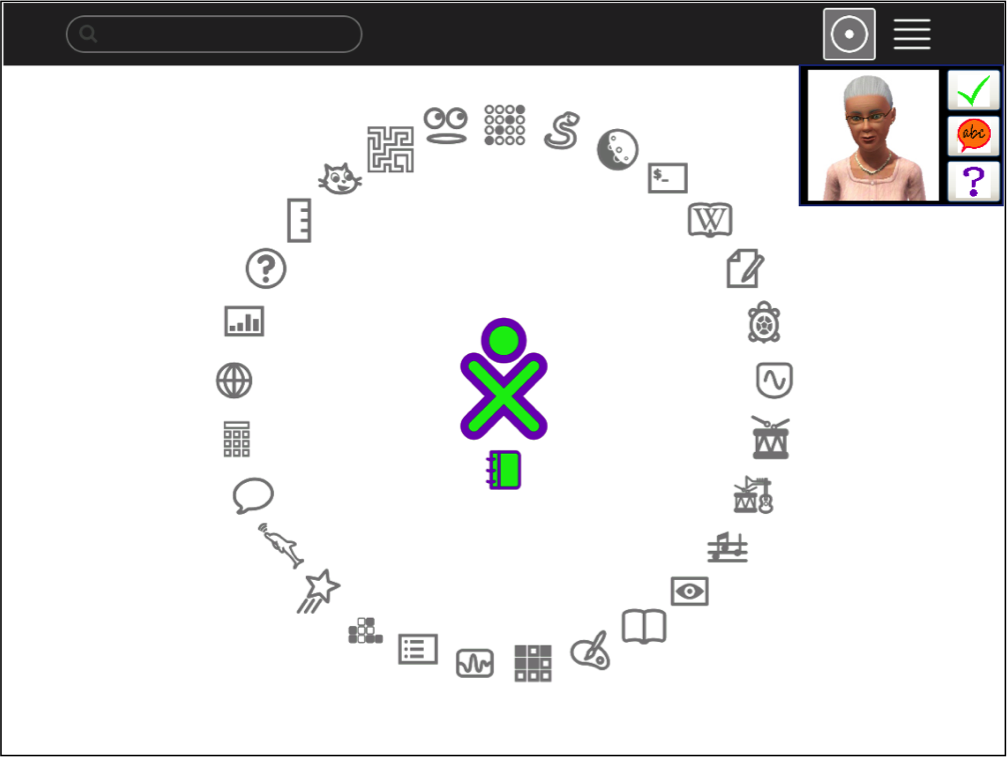
\includegraphics[width=0.7\textwidth]{intended-design.png}
\caption{Student interface design in SugarOS environment.}
\label{fig:intended-design}
\end{center}
\end{figure}

\begin{figure}[ht]
\begin{center}
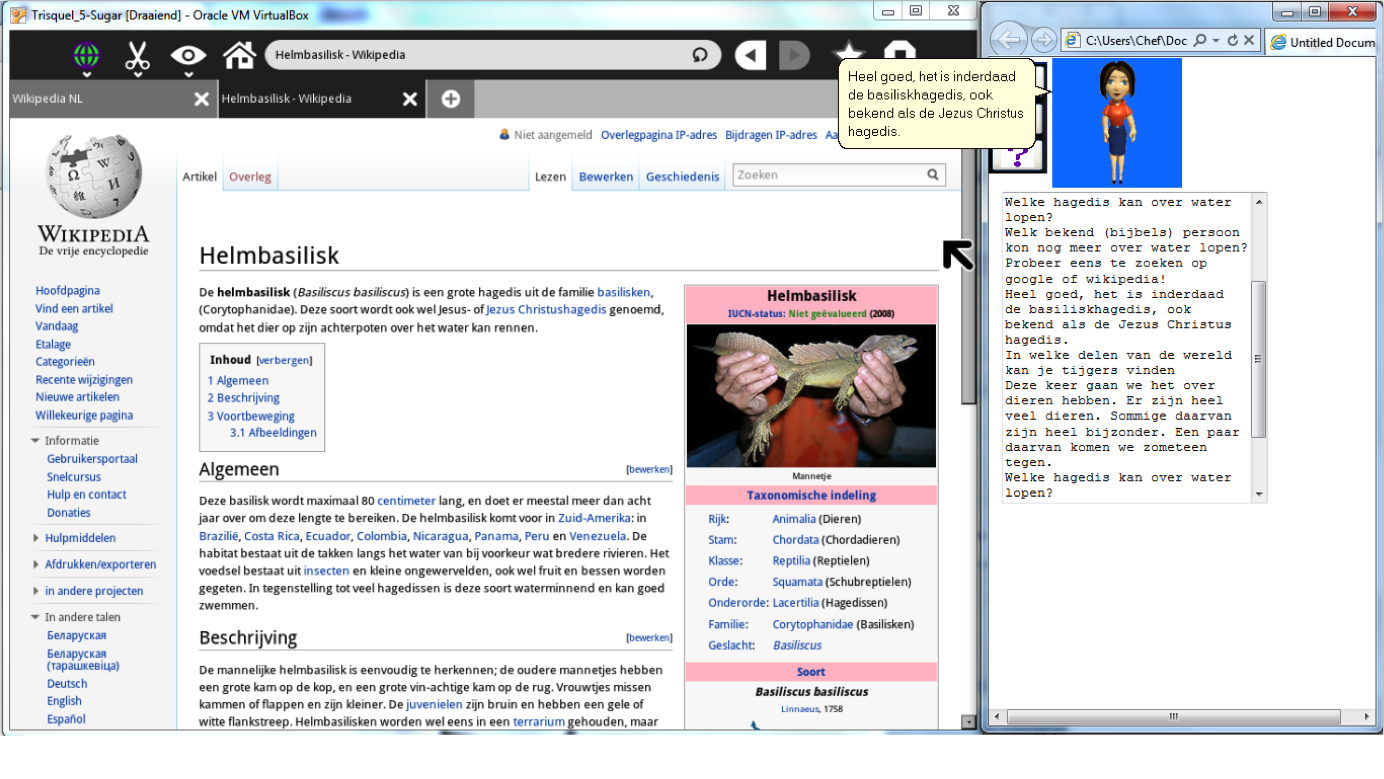
\includegraphics[width=0.7\textwidth]{pilot-design.png}
\caption{Design of a web-based pilot with SugarOS in a virtual machine.}
\label{fig:pilot-design}
\end{center}
\end{figure}

\section{Testing setup}

\subsection{Testing procedure} 

The testing procedure consisted of the following steps.

\begin{enumerate}
	\item Create a set of sample activities (in advance).
	\item Inform participants about the test.
	\item Provide the participants with a laptop with the installed environment and evaluate their behaviour while working with the OLE.
	\item Perform the questionnaire and the interview-based evaluation.
\end{enumerate}

\subsection{Testing claims}

Testing was intended to support or reject the following claims.

\begin{enumerate}
	\item The avatar motivates the user to learn about a certain topic and asks questions that allow the user to reflect on his progress thus improving learning experience.
	\item While using the OLE the user gains more knowledge about the world and understands it better. 
	\item Working in groups may increase the learning rate as this introduces a social aspect as well.
\end{enumerate}

\subsection{Testing objectives}

During the testing phase, we wanted to evaluate the approach and detect the usability problems. The main question concerning the learning approach we wanted to answer was whether the young children are in principle able to study by themselves using the computer and our virtual assistant. For detecting the problems in usability, we wanted to analyse how the participants interact with the system. We were interested whether the interaction is done in a pre-defined way and what functionality is missing.

\subsection{User experience measurements}

During the testing we tried to measure the following user experience aspects:

\begin{itemize}
	\item Encouragement: do students find it interesting to work with the assistant and complete the suggested challenges?
	\item Usability: do students feel themselves comfortable while working with the system or it is counter-intuitive/complex/etc.?
	\item Group work: do students find it more educational/fun to work in groups? 
\end{itemize}

\section{Testing results}

We performed two stages of testing the application. During the first stage, we used a focus group consisting of seven TU Delft students. Three of them worked on their own, four remaining persons were split into two groups. In the second phase we worked at the TU Delft Science Centre with fourteen children aged from 6 to 15 years either working on their own or in groups of two and three. During the first stage, all the participants worked with the avatar-enabled environment, and in the second stage four of the participants worked with a setup not containing the avatar and used only textual interaction with OLE. 

The general feedback from the focus groups was rather positive but it showed that the avatar needs to be improved.

The main results obtained after performing the tests are the following.

\begin{itemize}
	\item Those participants who used the prototype with the avatar had a significantly better attitude towards the program than participants who did not have the avatar in their setup.
	\item Almost all participants were able to answer all the questions. 
	\item Sample challenges that were used in the testing were designed to be quite straightforward. We feel that more open questions would lead to more curiosity and exploration. 
	\item The participants tended to associate the avatar with themselves, asking "is it me?".
	\item Female participants were significantly ($p < .05$) more positive towards the avatar. We relate it with the gender of the avatar and expect males to give a higher rating for the male avatar, allowing the participants to identify themselves with the avatar.
	\item We noticed that for young children the parents can take on the role of �grannie�.
	\item The hints issued by the avatar were sometimes confusing, mostly because the avatar was giving them unprovoked, based on the timings. Some participants claimed that the hints were given too fast, some claimed that the avatar was too slow. Ideally the display of the hints should be determined by the abilities of the students.
	\item Appearance of the new portion of a text (containing a new challenge or a hint) was often not detected.
	\item Individuals were mostly focused on the questions themselves and tried just to find an answer and go further. While working in groups, the participants used their time also to study the additional information about the topic and generally performed better.
	\item Girls were more inclined to explain things to each other while the boys tried to solve all the challenges as fast as possible.
	\item When working in a group, even if one participant knew the answer the group still used the internet to check the answer.
	\item While using the avatar in a group seemed to work well, it might be needed to encourage additional communication between group members with the help of the avatar.
	\item When working in a group, the �smartest� of the group tended to take the control. Less experienced group members should be involved more.
	\item Some participants got sidetracked and started showing us shark pictures.
	\item A number of interface-related remarks were issued. 
\end{itemize}

We can conclude that the first two of our claims were validated and the last one about the groups performing better than individuals may be correct, but it does not immediately follow from the results. This could possibly be validated when performing tests with a larger focus group.

\section{Recommendations}

The research performed by our group has clearly shown that the learning environments similar to the one developed within our project are useful in the organisation of self-organised group-based learning processes and this direction needs to be developed further. We issue the following recommendations that can be useful to the researchers interested in continuing our work.

\begin{itemize}
	\item The functionality of the Microsoft Agent assistant that we used in our pilot turned out to be insufficient for the use in real environments. It is recommended to use more advanced systems, i.e. WorldViz Vizard\footnote{http://www.worldviz.com/products/vizard/index.html}.
	\item To facilitate the best possible interaction with the students, face-only avatars with rich facial expressions are to be used.
	\item The quality of a text-to-speech engine is one of the keys to success.
	\item Beta-testing on a larger focus groups has to be performed to get better feedback.  
\end{itemize}

\section{Unresolved challenges}

While working on the project we faced a number of important questions that are to be answered in further research on the topic.

\begin{itemize}
	\item What mechanisms are to be used for retrieving the feedback, especially for process-oriented questions not requiring students to provide the exact answers?
	\item How can the localisation issues be dealt with? As our setup is different from what Sugata Mitra uses, we apparently cannot stick to English only. There should be a way to translate activities and filter them by language.
	\item How do such characteristics of an avatar as gender, age and pose affect the study process and the results?
	\item Which group sizes perform best?
\end{itemize}

\section{Conclusions}

During the project implementation we have built a pilot version of a learning environment that is intended to facilitate self-organised group-based learning process with the help of internet-connected computers for the unexperienced children not having any computer experience. The results that we achieved indicate that a virtual avatar can indeed become a valuable assistant for our setup and the research in the field of building the learning environments including such assistants has to be continued.

\begin{thebibliography}{99}
\bibitem{Cowell} Cowell, A.J., and Stanney, K.M. (2005). Manipulation of non-verbal interaction style and demographic embodiment to increase anthropomorphic computer character credibility. \emph{Int. J. Human-Computer Studies}, \#62,  pp. 281--306.
\end{thebibliography}

\appendix

\newpage

\section{Questionnaire}

To evaluate the built pilot, we used a questionnaire consisting of seven questions, each accepting an answer in range 1--5 with 5 being the most positive impression, 1 being the most negative impression. The answering scale was represented as emoticons with different expressions and we asked the participants to make a mark on the best suiting emoticon.

The questions were the following.

\begin{enumerate}
	\item Did you like the programme?
	\item Did you learn something new using it?
	\item Do you want to keep learning with this programme? 
	\item Was it easy to learn with it?
	\item Did you like the avatar?
	\item Was it easy to understand what is required from the avatar?
	\item Do you think the avatar helped you?
\end{enumerate}

\section{Gathered data}

The answers to the questionnaire that were gathered during the second phase of testing are presented in the table below.

\begin{center}
  \begin{tabular}{| c | c | c | c | c | c | c | c | c | c | c | c | c |}
    \hline
    \# & Group size & \# group & Gender & Avatar & Grade & Q1 & Q2 & Q3 & Q4 & Q5 & Q6 & Q7 \\ \hline
    
    1 & 1 &	-1 & F & + & 4 & 5 & 4 & 5 & 5 & 4 & 3 & 4 \\ \hline

    2 & 3 &  1 & F & + & 5 & 5 & 5 & 5 & 5 & 3 & 3 & 4 \\ \hline

    3 & 3 & 1 & F & + & 7 & 5 & 5 & 5 & 5 & 3 & 3 & 4 \\ \hline

 	4 & 3 & 1 & F & + & 7 & 5 & 5 & 4 & 3 & 3 & 3 & 4 \\ \hline

 	5 & 2 & 2 & M & + & 7 & 4 & 4 & 5 & 5 & 5 & 5 & 4 \\ \hline

 	6 & 2 & 2 & M & + & 8 & 5 & 4 & 5 & 4 & 5 & 4 & 3 \\ \hline

 	7 & 2 & 6 & M & - & 3 & 3 & 1 & 1 & 5 & -1 & -1 & -1 \\ \hline

 	8 & 2 & 6 & F & - & 5 & 3 & 4 & 2 & 1 & -1 & -1 & -1 \\ \hline

 	9 & 3 & 5 & M & + & 6 & 5 & 5 & 5 & 4 & 4 & 5 & 4 \\ \hline

 	10 & 3 & 5 & M & + & 6 & 4 & 4 & 3 & 5 & 4 & 5 & 3 \\ \hline

 	11 & 3 & 5 & M & + & 5 & 4 & 5 & 4 & 5 & 4 & 4 & 3 \\ \hline

	12 & 2 & 3 & F & - & 10 & 4 & 3 & 4 & 3 & -1 & -1 & -1 \\ \hline

 	13 & 2 & 3 & F & - & 10 & 4 & 2 & 3 & 4 & -1 & -1 & -1 \\ \hline

 	14 & 1 & -1 & F & + & 7 & 4 & 5 & 5 & 4 & 4 & 5 & 4 \\ \hline
  \end{tabular}
\end{center}

\section{ANOVA}

We conducted an ANOVA to see if having an avatar present in the prototype influenced the aggregated attitude measure, which was  determined by taking the means of the 5 point Likert-scale questions on the program in general (See the Appendix A for the full questionnaire).

The results of this ANOVA showed that those participants who used the prototype with the avatar had a significantly ($F(1,12) =  54.784, p < .001$) better attitude towards the program than participants who did not have the avatar. The boxplot shown at Figure~\ref{fig:boxplot-avatar} shows that the mean of the score given by participants who used the version with the avatar is around 1.25 points higher than the score given without the avatar.\newline

\begin{center}
  \begin{tabular}{| c | c | c | c | c | c |}
    \hline
    Attitude & Sum squares & df & Mean square & F & Sig. \\ \hline
    
    Between groups & 7.661 & 1 & 7.661 & 54.784 & .000 \\ \hline

    Within groups & 1.678 & 12 & .140 & & \\ \hline

    Total & 9.339 & 13 & & & \\ \hline
  \end{tabular}
\end{center}

Another ANOVA was conducted to look at the relationship between gender and the answers given on the questionnaire. While no significant effects were found for the first four questions regarding the prototype in general, there was a significant effect ($p < .05$) on the questions regarding the avatar itself. The data shows that female participants consistently rated the avatar higher than the males did. This seems to indicate that children prefer to be taught by a teacher or avatar of their own gender, so that they can more easily identify themselves with the avatar. However, for us to be able to conclude this, additional research using different avatars is needed.

\begin{center}
  \begin{tabular}{| c | l | c | c | c | c | c |}
    \hline
    Question & Attitude & Sum squares & df & Mean square & F & Sig. \\ \hline
    
    Q1 & Between groups & .149 & 1 & 149 & .266 & .615  \\ \hline
    & Within groups & 6.708 & 12 & .559 &  &  \\ \hline
    & Total & 6.857 & 13 &  &  &  \\ \hline


    Q2 & Between groups & .292 & 1 & .292 & .178 & .681  \\ \hline
    & Within groups & 19.708 & 12 & 1.642 & &  \\ \hline
    & Total & 20.000 & 13 &  &  &  \\ \hline

    Q3 & Between groups & .292 & 1 & .292 & .161 & .695 \\ \hline
    & Within groups & 21.708 & 12 & 1.809 & &  \\ \hline
    & Total & 22.000 & 13 &  &  &  \\ \hline

    Q4 & Between groups & 2.881 & 1 & 2.881 & 2.331 & .153 \\ \hline
    & Within groups & 14.833 & 12 & 1.236 & &  \\ \hline
    & Total & 17.714 & 13 &  &  &  \\ \hline

    Q5 & Between groups & 2.500 & 1 & 2.500 & 8.333 & .020 \\ \hline
    & Within groups & 2.400 & 8 & .300 &  &  \\ \hline
    & Total & 4.900 & 9 &  &  &  \\ \hline

    Q6 & Between groups & 3.600 & 1 & 3.600 & 6.545 & .034 \\ \hline
    & Within groups & 4.400 & 8 & .550 &  &  \\ \hline
    & Total & 8.000 & 9 &  &  &  \\ \hline

    Q7 & Between groups & .900 & 1 & .900 & 6.000 & .040 \\ \hline
    & Within groups & 1.200 & 8 & .150 &  &  \\ \hline
    & Total & 2.100 & 9 &  & &  \\ \hline

  \end{tabular}
\end{center}

\begin{figure}[ht]
\begin{center}
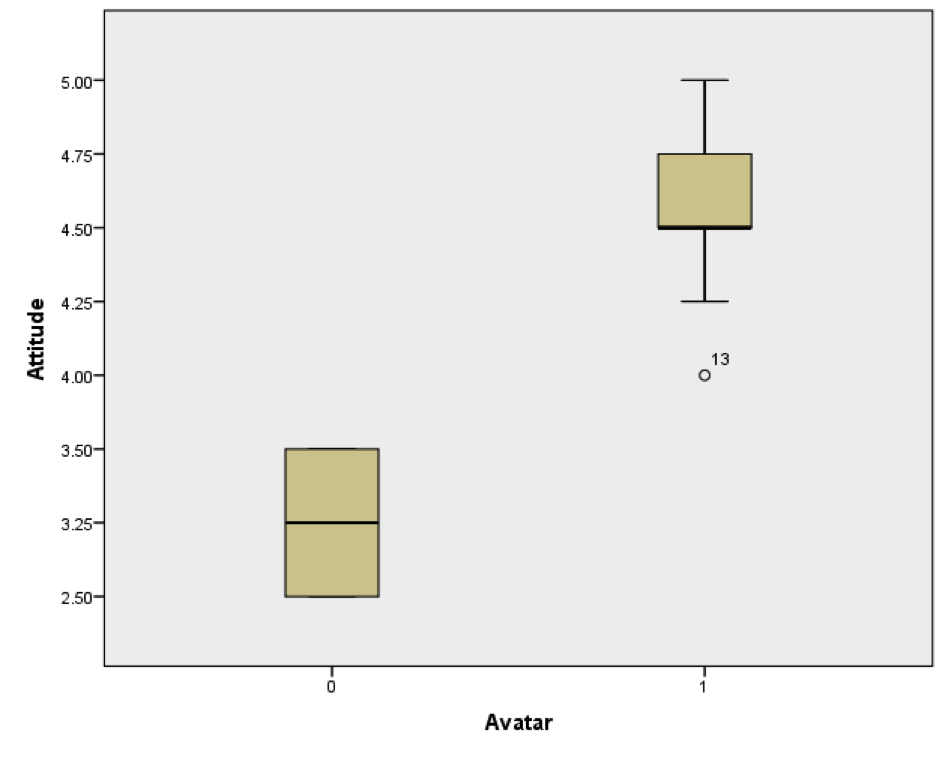
\includegraphics[width=0.7\textwidth]{boxplot-avatar.png}
\caption{Boxplot of the aggregated attitude measure for the prototypes with and without the avatar.}
\label{fig:boxplot-avatar}
\end{center}
\end{figure}

\begin{figure}[ht]
\begin{center}
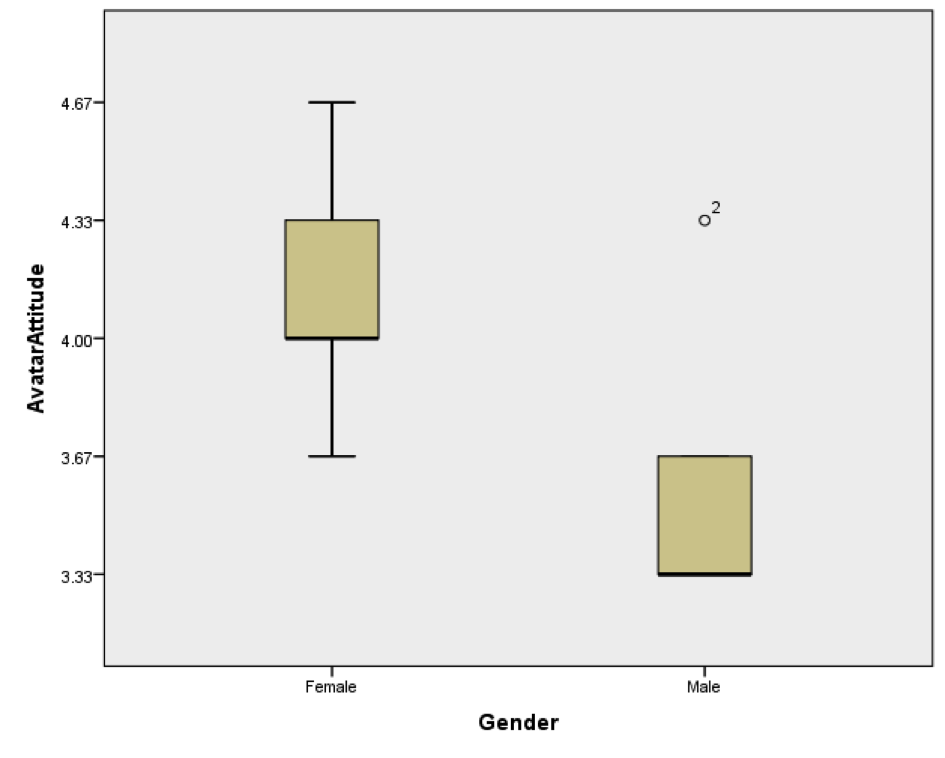
\includegraphics[width=0.7\textwidth]{boxplot-gender.png}
\caption{Boxplot of the aggregated avatar attitude measure for female and male participants.}
\label{fig:boxplot-gender}
\end{center}
\end{figure}

\end{document}